\section{Methodology}
\label{sec:methodology}

The general approach taken for analyzing HPC code-bases was to extract dependency data from each file, create a directed weighted graph of the dependencies between the files, and use a clustering algorithm to identify key architectural structures in the graph. A visual overview of this process can be seen in Figure \ref{fig:workflow} and will be described in more detail throughout the rest of this section. The specific middlewares test using this methodology are covered in Section \ref{subsec:workloads}.

\begin{figure*}[ht]
    \centering
    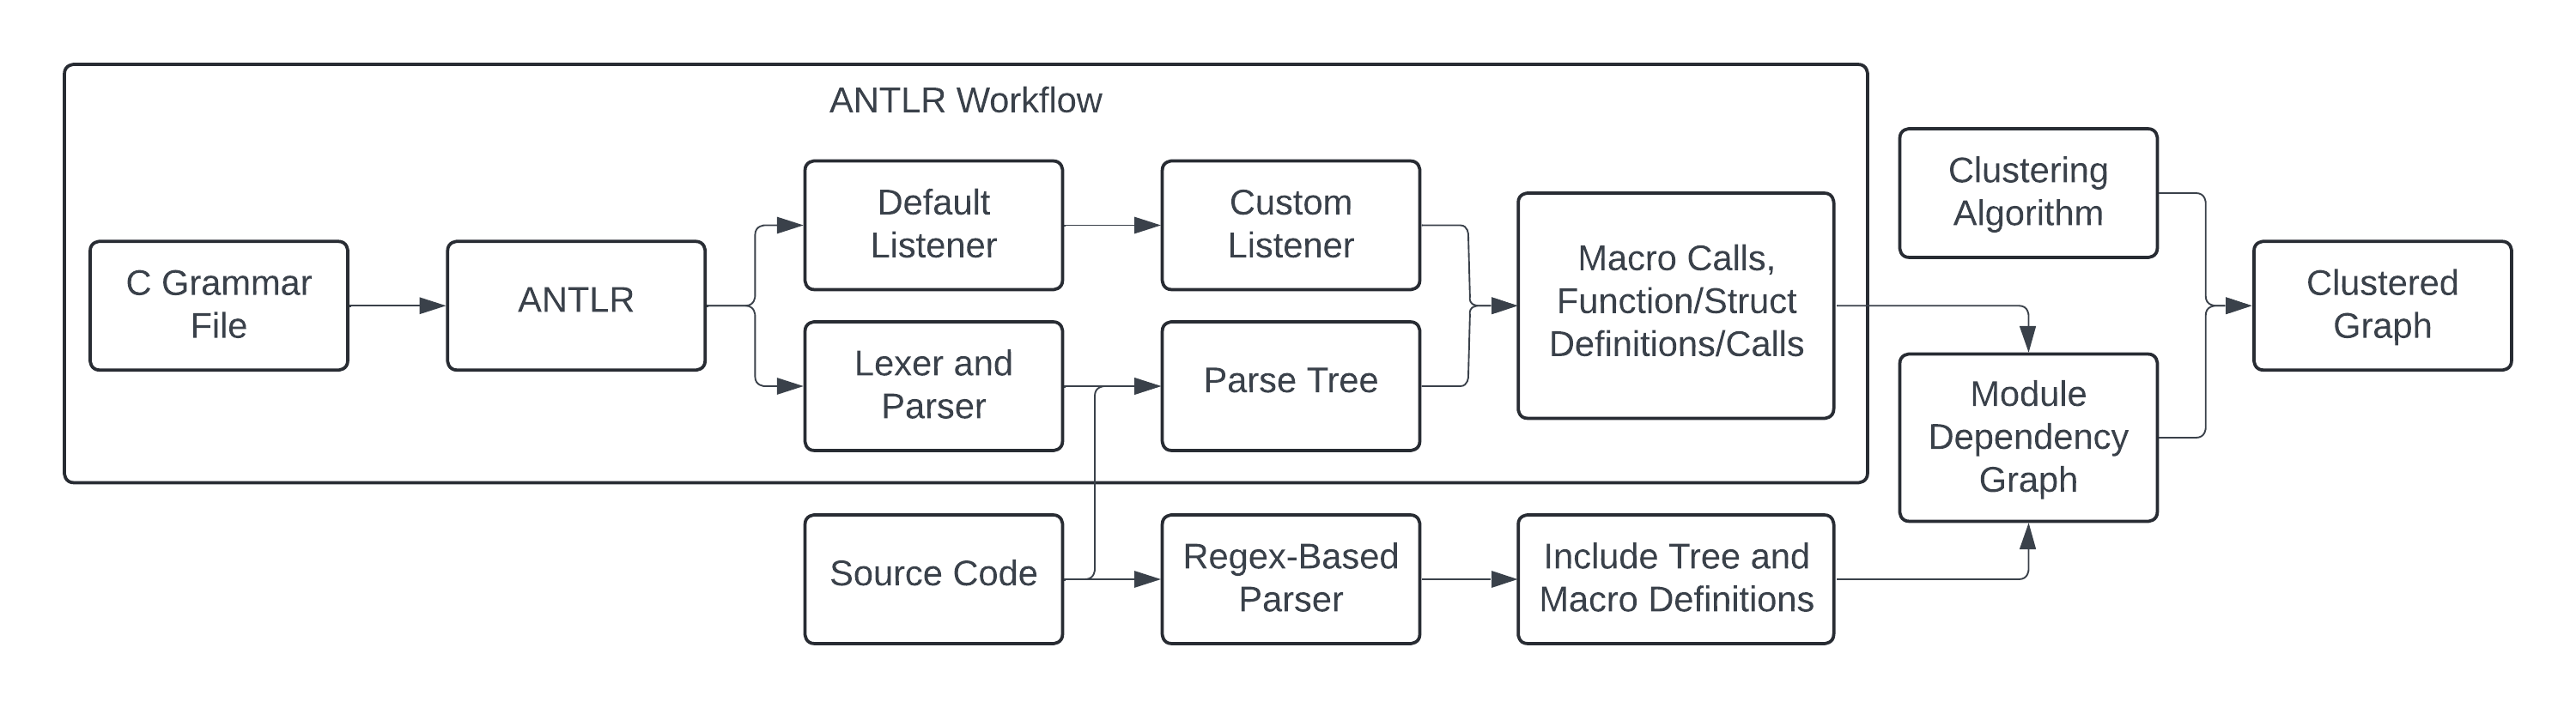
\includegraphics[width=1.0\linewidth]{figures/workflow_diagram.png} \\
    \caption{A diagram of the workflow used for the analysis of HPC code-bases.}
    \label{fig:workflow}
\end{figure*}
